




\paragraph{Description of the model}
Two Higgs doublet models provide natural, consistent embeddings of scalar and pseudoscalar mediators to a dark sector. Besides the SM scalar $h$, it predicts a neutral scalar $H$, a charged scalar $H^\pm$, and a pseudoscalar spin-0 state $A$. Several shortcomings and unmotivated assumptions in the simplified model are remedied in this framework. Couplings between SM fermions and the physical (pseudo)scalar are renormalizable. The custodial symmetry of the SM electroweak sector is protected at tree-level and therefore contributions to electroweak precision observables are loop-suppressed. Flavour- and CP-changing neutral currents are protected at tree-level if a discrete symmetry is imposed on the two scalar doublets $H_1$ and $H_2$, under which $H_1\to H_1$ and $H_2\to -H_2$. This $Z_2$ symmetry is the minimal condition necessary to guarantee the absence of FCNCs at tree-level \cite{Glashow:1976nt,Paschos:1976ay} and such a symmetry is realized in many well-motivated complete ultraviolet theories in the form of supersymmetry, a $U(1)$ symmetry or a discrete symmetry acting on the Higgs doublets. The Yukawa structure of 2HDMs differentiate between the different types, 
\begin{equation} \label{eq:LY}
{\cal L}_{Y} = - \sum_{i=1,2} \left ( \bar Q Y_u^i \tilde H_i u_R  + \bar Q Y_d^i H_i d_R   + \bar L Y_\ell^i H_i \ell_R  + {\rm h.c.}  \right ) \,,
\end{equation}
and we collect the different models in Table \ref{tab:coeffs} below. The signatures discussed in this paper are largely independent of the type of 2HDM, but different signatures are more or less prominent depending on the Yukawa structure. Minimal flavour violating Yukawa structures with an explicitly broken $Z_2$ symmetry allow for additional decay channels and collider signatures. 
%
\begin{table}[b]\centering
\begin{tabular}{|c|c|c|c|}
\hline
Model & up-type & down-type & leptons
\\ \hline
Type I & $H_2$ & $H_2$ & $H_2$
\\
Type II & $H_2$ & $H_1$ & $H_1$
\\
Type III (X) & $H_2$ & $H_2$ & $H_1$
\\
Type IV (Y) & $H_2$ & $H_1$ & $H_2$
%\\
%Inert & - & - &-
\\ \hline
\end{tabular}
\caption{Categorization of the different Yukawa sectors for models with discrete ${Z}_2$
  symmetries. The two Higgs doublet models of Type III and IV are also called Type X and Y or \emph{lepton-specific} and \emph{flipped} in the literature. }\label{tab:coeffs}
\end{table}
In general, the presence of vacuum expectation values $\langle H_i\rangle=(0,v_i/\sqrt{2})^T$, breaks the $Z_2$ symmetry. If the vacuum respects the $Z_2$ symmetry, \emph{i.e.} one of the vevs vanishes, the corresponding Higgs doublet is \emph{inert}. The lightest component of this doublet is stable and provides a natural DM candidate \cite{}. The inert 2HDM is a elegant, consistent model of scalar DM as a component of an $SU(2)_L$ doublet. For more general DM candidates, the coupling of the physical (pseudo)scalar to DM requires additional assumptions. For a SM singlet, Dirac fermion $\chi$, the operators $\bar \chi \chi$ and $\bar \chi \gamma_5\chi$ are singlets and renormalizable couplings to $H_1$ or $H_2$ are not possible. For the physical (pseudo)scalar to be a mediator to a dark sector, either additional $SU(2)_L$ doublet fermions or $SU(2)_L$ singlet scalars are necessary. If these degrees of freedom are decoupled from the spectrum, one can consider dimension five couplings to DM
\begin{align}
\mathcal{L}=\frac{H_1^\dagger H_2}{\Lambda} \bar \chi \chi+\frac{H_1^\dagger H_2}{\Lambda} \bar \chi \gamma_5 \chi + \emph{h.c.}\,,
\end{align}
in which $\Lambda \gg v$ denotes the mass scale of these additional states. This framework captures the universal properties of such a (pseudo)scalar mediator \cite{}. If the additional states are light, $\Lambda \lesssim v$, additional signatures allow to distinguish the mediator structure. We focus on a class of models with an additional, real singlet, which either transforms as a scalar $S$ or pseudoscalar $P$ with DM couplings
%
\begin{align} \label{eq:Lx}
{\cal L}_{P\chi} &= - i \hspace{0.25mm} y_\chi P \hspace{0.25mm} \bar \chi \hspace{0.25mm} \gamma_5 \hspace{0.1mm} \chi \,,\\
{\cal L}_{S\chi} &= -  \hspace{0.25mm} y_\chi S \hspace{0.25mm} \bar \chi   \chi \,,
\end{align}
%
It is straightforward to embed the real scalar $S$ and pseudoscalar $P$  a complex field $\phi = S+i P$, and a potential vev of $S$ can contribute to the DM mass \cite{}. \\

\paragraph{Pseudoscalar Mediator} 
In order to identify the CP eigenstates with the mass eigenstates, two scalars $h$ and $H$, two pseudoscalars $a$ and $A$, and a charged scalar $H^\pm$, we choose all parameters of the scalar potential real. The most general scalar potential can be written as 
\begin{align}\label{eq:fullPot}
V(P,H)=V_H+V_{PH}+V_P\,,
\end{align}
with the potential for the two Higgs doublets
\begin{align}\label{eq:VH}
V_{H} & = \mu_1 H_1^\dagger H_1 + \mu_2 H_2^\dagger H_2 + \left ( \mu_3  H_1^\dagger H_2 + {\rm h.c.} \right ) + \lambda_1  \hspace{0.25mm} \big ( H_1^\dagger H_1  \big )^2  + \lambda_2  \hspace{0.25mm} \big ( H_2^\dagger H_2 \big  )^2 \notag \\
& \phantom{xx} +  \lambda_3 \hspace{0.25mm} \big ( H_1^\dagger H_1  \big ) \big ( H_2^\dagger H_2  \big ) + \lambda_4  \hspace{0.25mm} \big ( H_1^\dagger H_2  \big ) \big ( H_2^\dagger H_1  \big ) + \left [ \lambda_5   \hspace{0.25mm} \big ( H_1^\dagger H_2 \big )^2 + {\rm h.c.} \right ]  \,,
\end{align}
potential terms which connect doublets and singlets 
\begin{equation} \label{eq:VHP}
\begin{split}
V_{HP}  = P \left ( i \hspace{0.1mm} b_P  \hspace{0.1mm}  H_1^\dagger H_2 + {\rm h.c.} \right ) + P^2 \left (  \lambda_{P1}  \hspace{0.1mm}  H_1^\dagger H_1 +   \lambda_{P2}  \hspace{0.1mm}  H_2^\dagger H_2 \right )  \,,
\end{split} 
\end{equation}
and the singlet potential
\begin{equation} \label{eq:VP}
V_{P}  =  \frac{1}{2} \hspace{0.5mm} m_P^2  P^2 +  \lambda_P\,P^4 \,.
\end{equation}
Upon rotation to the mass eigenbasis, we trade the five dimensionful and eight dimensionless parameters in the potential  for physical masses and mixing angles and three quartic couplings
\begin{align}
\left\{ \,\,\begin{matrix}
\mu_1,\,\mu_2,\\[3pt]
\mu_3\,, m_P^2,\, b_P\\[3pt]
\lambda_1\,,\lambda_2\,,\lambda_3\,,\lambda_4\,,\lambda_5\\
\lambda_{P1}\,,\lambda_{P2} \,, \lambda_P
\end{matrix}\,\,\right\}\qquad \quad \longleftrightarrow \quad \qquad \left\{ \,\,\begin{matrix}
v,\, M_h,\,\cos(\beta-\alpha)\\[3pt]
M_a\,, M_A\,, M_H\,,M_{H^\pm}\\[3pt]
t_\beta\,, \cos(\theta)\,, \\[3pt]
\lambda_3\,,\lambda_{P1}\,,\lambda_{P_2}\,,\lambda_P
\end{matrix}\,\,\right\}\,.
\end{align}
Out of these parameters, the electroweak scale $v=246$ GeV and the mass of the SM-like CP-even mass eigenstate $M_h=125$ GeV are fixed. The mixing angle $\alpha$ between the CP-even scalars $h$ and $H$ is constrained by Higgs coupling strength measurements \cite{} and we show the allowed parameter space in the $\cos(\beta-\alpha)$ plane in  Fig.~\ref{fig:higgsfit} for the Yukawa sector of a 2HDM of type II.  For arbitrary values of $t_\beta=v_2/v_1$ only the limit $\cos(\beta-\alpha)\approx 0$ is allowed, for which the couplings of the CP-even state $h$ align with the couplings of the SM Higgs boson. For the analyses discussed in the remainder of this paper, we choose this so-called alignment limit and treat $t_\beta$ as a free parameter.
%%
\begin{figure}[t]
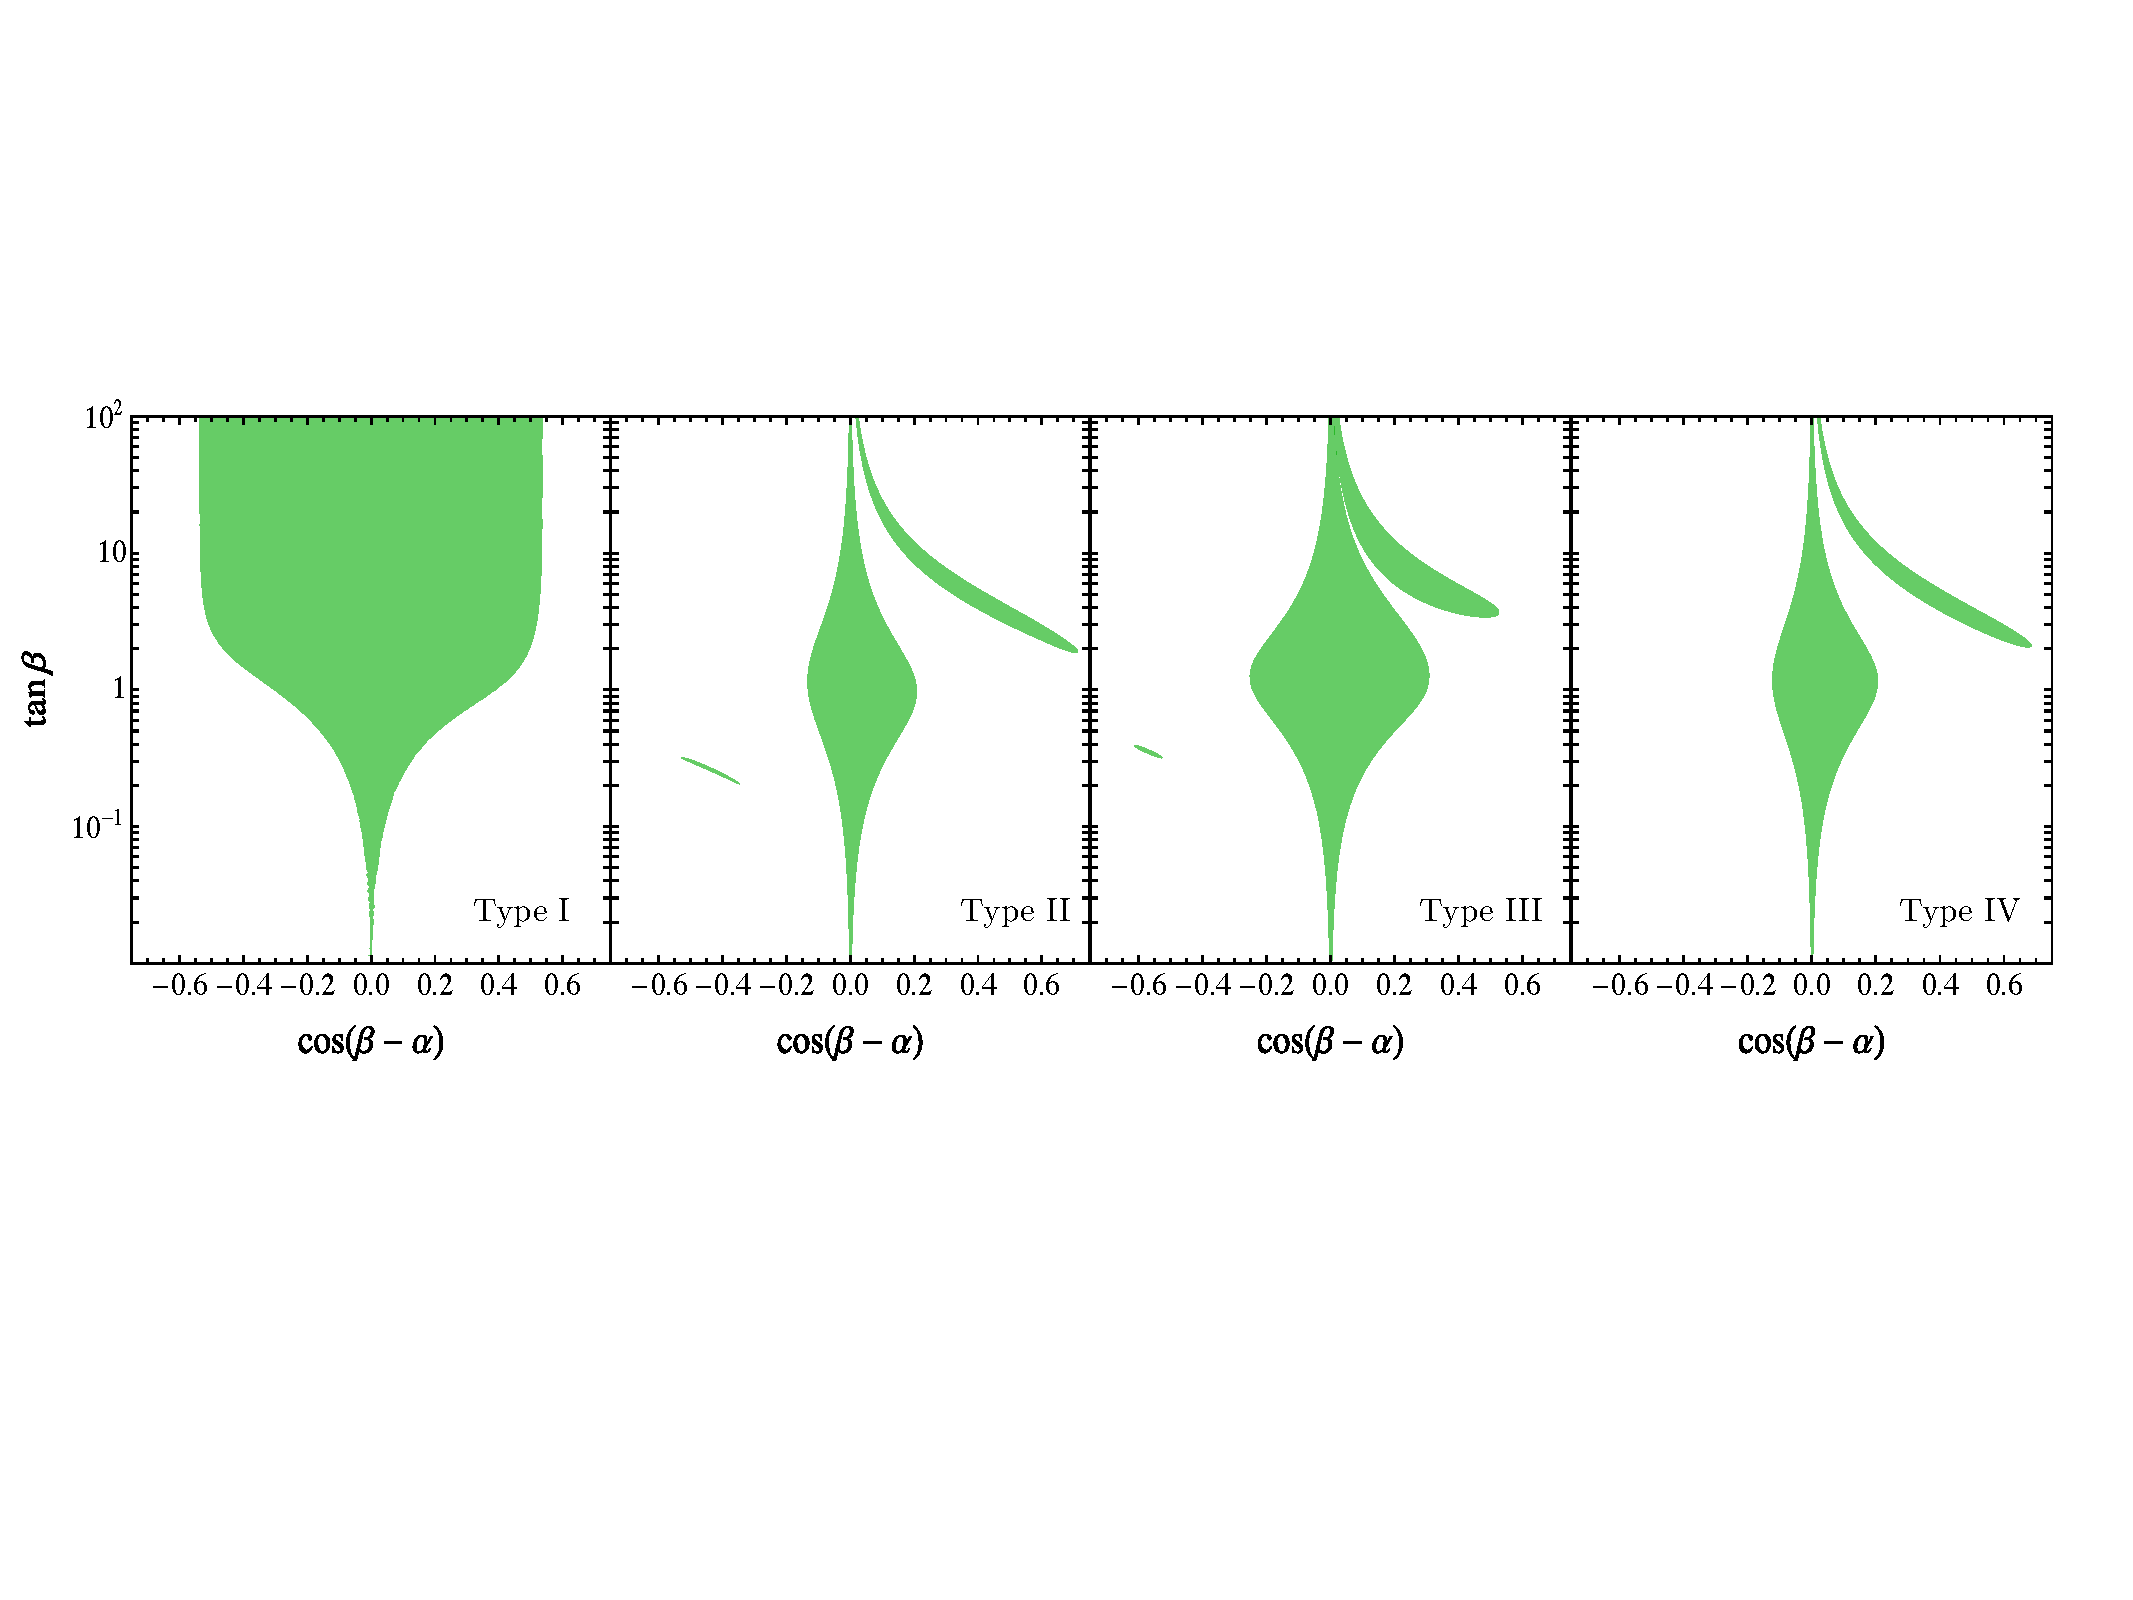
\includegraphics[width=\textwidth]{Figs/Higgsfit}
\caption{\label{fig:higgsfit} Parameter space allowed by a global fit to Higgs coupling strength measurements for (from left to right) a Yukawa sector of type I ($Y_u^1  = Y_d^1 = Y_\ell^1 =0$), type II ($Y_u^1 = Y_d^2 = Y_\ell^2 =0$),  type III ($Y_u^1 = Y_d^1 = Y_\ell^2 =0$), and type IV ($Y_u^1  = Y_d^2 = Y_\ell^1 =0$). }
\end{figure}
%%
Electroweak precision measurements constrain the splitting between the masses $M_H, M_A, M_a$ and $M_{H^\pm}$, since loops of spin-0 states modify the propagators of the electroweak gauge bosons at one-loop. For $M_H=M_{H^\pm}$ and $\cos(\beta-\alpha)=0$, these corrections vanish due to a custodial symmetry in the tree-level potential $V_H$ \cite{} and the masses of the CP-odd mass eigenstates can be treated as free parameters. This custodial symmetry is also present in $V_H$ if $M_A=M_{H^\pm}$ and $\cos(\beta-\alpha)=0$, but the presence of the pseudoscalar mixing term in $V_P$ softly breaks this symmetry. As a consequence, the pseudoscalar mixing angle $\theta$ and the mass splitting between $M_H$, $M_A$ and $M_a$ are constrained in this situation. In Fig.~\ref{fig:EWPM}, we show these constraints as maximally allowed $\sin \theta$ contours in the $(M_a, M_H)$ plane.
Flavour observables are mostly sensitive to corrections from one-loop exchanges of the charged scalar ${H^\pm}$, whose contributions to $b \to X_s \gamma$ \cite{Hermann:2012fc,Misiak:2015xwa,Czakon:2015exa} and $B_s-\bar B_s$ mixing \cite{Abbott:1979dt,Geng:1988bq,Buras:1989ui,Eberhardt:2013uba} lead to the strongest indirect constraints on $M_{H^\pm}$. Since the couplings of the charged scalar only depend on $t_\beta$, these constraints result in the bound $\tan \beta \gtrsim 0.8$ for $M_{H^\pm}=750$ GeV, independent of the choice of the Yukawa sector.\\
%%
\begin{figure}[t]
\centering
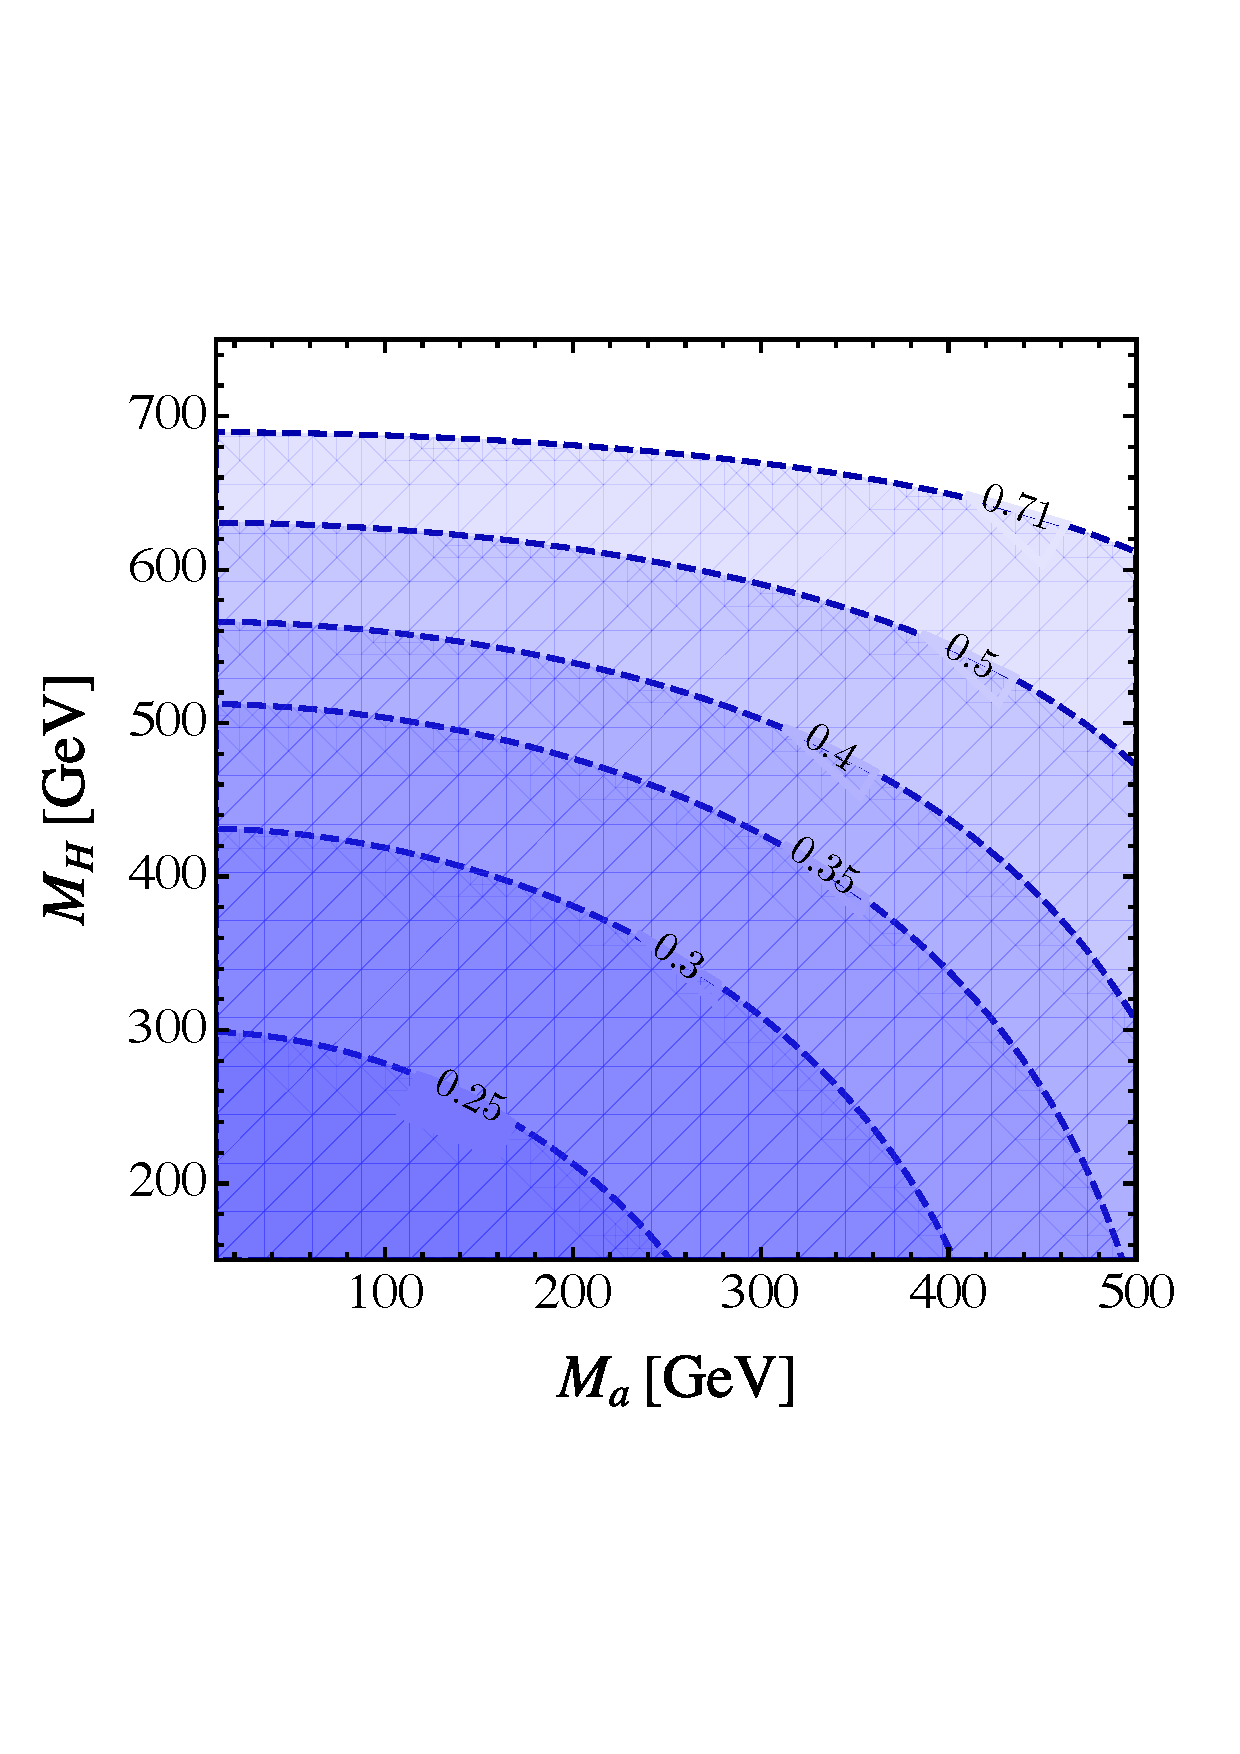
\includegraphics[width=.5\textwidth]{Figs/EWPM}
\caption{\label{fig:EWPM}Values of $M_H$ and $M_a$ allowed by electroweak precision constraints for $\cos(\beta-\alpha)=0, M_{H^\pm}=M_A=750$ GeV, and varying values of the pseudoscalar mixing angle $\sin \theta =0.25, 0.3, 0.35, 0.4, 0.5$ , and maximal mixing angle $\sin\theta =1/\sqrt{2}\approx 0.71$. The parameter space below and to the left of the dashed contours is excluded. The same plot can be produced for the scalar mediator model for $\cos(\beta-\alpha)=0, M_{H^\pm}=M_H=750$ GeV by exchanging $M_a\rightarrow M_{S_1}$ and $M_H\rightarrow M_{A}$. }
\end{figure}
%%
In addition to these constraints, the potential $V_H$ needs to give rise to a stable vacuum breaking the electroweak symmetry, whereas the parameters in $V_P$ need not introduce a vacuum expectation value for $P$, and scattering amplitudes should remain perturbative \cite{Gunion:2002zf,Barroso:2013awa} and unitary \cite{Kanemura:1993hm,Akeroyd:2000wc,Ginzburg:2005dt,Grinstein:2015rtl} up to the UV scale, where the 2HDM+a is UV completed.  These conditions impose additional constraints on the quartic couplings in the potential, which are satisfied for $M_H, M_A, M_a \lesssim \mathcal{O}(1)$ TeV and $\lambda_3, \lambda_{P1}, \lambda_{P2}$ and $\lambda_P$ of $\mathcal{O}(1)$ as long as $t_\beta$ is not too much smaller than one. For the case of fixed\footnote{The singlet quartic $\lambda_P$ is entirely irrelevant for the phenomenology of the 2HDM+a.} $\lambda_3, \lambda_{P1}, \lambda_{P2}$, the stability condition therefore leads to additional constraints on the mixing angle $\theta$ and the masses. The parameter space of the 2HDM+a is strongly constrained, as summarized below.
%
\newline
\begin{tabular}{cc c}
&&\\
$v, M_h, \cos(\beta-\alpha) $&$\longleftrightarrow$& fixed by Higgs measurements,\\[.3cm]
$M_{H^\pm}\,, $  &$\longleftrightarrow $& constrained by flavour observables,\\[.3cm]
$\sin(\theta)\,, M_H \,\,\text{or} \,\,M_A$  &$\longleftrightarrow $& constrained by EWPM,\\[.3cm]
$\lambda_3, \lambda_{P1}, \lambda_{P2}\,,\lambda_P $ &$\longleftrightarrow $& constrained by stability, perturbativity and unitarity constraints\,.\\[.3cm]
&&
\end{tabular}
\newline
%
This leaves us with effectively three free parameters from the potential, the Dark Matter mass and the coupling of the mediator to the DM candidate
\begin{align}
\big\{ m_\chi\,,\,\,M_a\,,\,\, t_\beta\,, \,\, M_H\,\,\text{or}\,\,M_A\,\,, \,\, y_\chi\,\big\}\,.
\end{align}



\paragraph{Scalar Mediator}
For a scalar mediator, the most general potential 
\begin{align}
V(S, H)= V_H + V_{SH} +V_S
\end{align}
can be conveniently given in the Higgs basis, which is defined by  
\begin{align}
\begin{pmatrix}
\Phi_h\\
\Phi_H
\end{pmatrix} =\begin{pmatrix}
\cos\beta & \sin \beta \\
-\sin\beta & \cos \beta 
\end{pmatrix}
\begin{pmatrix}
H_1\\
H_2
\end{pmatrix}\,,
\end{align}
such that  $\langle \Phi_H \rangle =0$ and $\langle \Phi_h\rangle=v$. In this basis, the potential in \eqref{eq:VH} is given by (we denote couplings and potentials in the Higgs basis by a hat)
\begin{align}
\hat{V}_{H} &= \hat{M}_{hh}^2 \Phi_h^\dagger \Phi_h + \hat{M}_{HH}^2 \Phi_H^\dagger \Phi_H +  (\hat{M}_{hH}^2 \Phi_H^\dagger \Phi_h + h.c.) + \frac{\hat{\lambda}_h}{2} (\Phi_h^\dagger \Phi_h)^2 + \frac{\hat{\lambda}_H}{2} (\Phi_H^\dagger \Phi_H)^2 \nonumber \\
&+\hat{\lambda}_3 (\Phi_h^\dagger \Phi_h)(\Phi_H^\dagger \Phi_H) + \hat{\lambda}_4 (\Phi_H^\dagger \Phi_h)(\Phi_h^\dagger \Phi_H)  
+ \frac{\hat{\lambda}_5}{2} \left( (\Phi_H^\dagger \Phi_h)^2 + h.c.\right),
\end{align}
the part which allows for mixing between the scalar singlets and doublets reads
\begin{align}
\hat{V}_{SH}&=
  S^2 \bigg( \frac{\hat{\lambda}_{hhs}}{2} \Phi_h^\dagger \Phi_h +  \frac{\hat{\lambda}_{HHS}}{2}(\Phi_H^\dagger \Phi_H)+\frac{1}{2}(\hat{\lambda}_{hHS} \Phi_H^\dagger \Phi_h + h.c.)\bigg) \,,
\end{align}
and the scalar singlet self-interaction is given by 
\begin{align}
\hat{V}_S &= \frac{1}{2} \hat{M}_{SS}^2 S^2 + \frac{1}{4} \hat{\lambda}_S S^4\,.
\end{align}
There are again 13 parameters, which can be exchanged for physical masses and mixing angles as well as a number of additional dimensionless parameters
\begin{align}
\left\{ \,\,\begin{matrix}
\hat M_{hh}^2,\,\hat M_{HH}^2,\\[3pt]
\hat M_{hM}^2\,, \hat M_{SS}^2,\\[3pt]
\hat\lambda_h\,,\hat\lambda_H\,,\hat\lambda_3\,,\hat\lambda_4\,,\hat \lambda_5\\
\hat \lambda_{hhS}\,,\hat \lambda_{HHS} \,, \hat\lambda_{hHS}\,,\hat\lambda_S
\end{matrix}\,\,\right\}\qquad \quad \longleftrightarrow \quad \qquad \left\{ \,\,\begin{matrix}
v,\, M_h,\,\cos(\beta-\alpha)\\[3pt]
M_{S_1}\,, M_A\,, M_{S_2}\,,M_{H^\pm}\\[3pt]
t_\beta\,, \cos(\theta)\,, \\[3pt]
\hat \lambda_4\,,\hat \lambda_{5}\,,\hat \lambda_{S}\,,\hat \lambda_{HHS}
\end{matrix}\,\,\right\}\,,
\end{align}
in which the additional neutral scalar state $S_1$ and $S_2$ are superpositions of $S$ and $H$.
Analogous to the case of a pseudoscalar mediator, several constraints reduce this number of parameters. Measurements of the 125 GeV Higgs mass and its couplings determine $v, M_h$ as well as $\cos(\beta-\alpha)\approx 0$ and $\hat \lambda_{hHS}\approx 0$. The latter condition leads to suppressed $h-S$-mixing. Constraints from electroweak precision measurements are very weak for $M_{H^\pm}=M_A$, in which the custodial symmetry is preserved, but relevant for $M_{H^\pm}=M_{S_2}$ and varying $M_{S_1}$. The calculation is exactly analogous to the pseudoscalar case for $M_H \leftrightarrow M_A$ and $M_a\leftrightarrow M_{S_1}$, and leads to the constraints shown in Fig.~\ref{figures/EWPM} for these replacements. Vacuum stability and perturbativity conditions constrain the quartic couplings and flavour observables are independent of the mediator structure and only depend on $M_{H^\pm}$. We summarize as before 
 %
\newline
\begin{tabular}{cc c}
&&\\
$v, M_h, \cos(\beta-\alpha), \hat{\lambda}_{hhS} $&$\longleftrightarrow$& fixed by Higgs measurements,\\[.3cm]
$M_{H^\pm}\,, $  &$\longleftrightarrow $& constrained by flavour observables,\\[.3cm]
$\sin(\theta)\,, M_{S_2} \,\,\text{or} \,\,M_A$  &$\longleftrightarrow $& constrained by EWPM,\\[.3cm]
$\hat \lambda_4, \hat \lambda_{5}, \hat \lambda_{S}\,,\hat \lambda_{HHS} $ &$\longleftrightarrow $& constrained by stability, perturbativity and unitarity constraints\,,\\[.3cm]
&&
\end{tabular}
\newline
%
 which apart from the fermion couplings leaves the effective parameters
 \begin{align}
\left\{m_\chi\,,\,\, M_{S_1}\,,\,\, t_\beta\,,\,\, M_{S_2}\,\, \text{or}  \,\, M_{A}\,, \,\, y_\chi \right\}\,.
\end{align}

\paragraph{The effect of the quartic self-couplings  }

    The conditions under which the tree-level potential \eqref{eq:fullPot} remains bounded from below are $\lambda_{P_1}, \lambda_{P_2}>0$ and ~\cite{Gunion:2002zf}:
    %
    \begin{equation}
    \label{stability2HDM}
     \lambda_1 > 0\,, \,\,\, \lambda_2 > 0\,, \,\,\, \lambda_3 > - \sqrt{\lambda_1 \lambda_2} \,, \,\,\, \lambda_3 + \lambda_4 - |\lambda_5| > - \sqrt{\lambda_1 \lambda_2} 
    \end{equation}
    %
    which can be inferred from analyzing the scalar potential at large field values $H_1,\,H_2 \gg v$. For $M_{H^{\pm}} = M_{H_0}$, the first two conditions 
    in~\eqref{stability2HDM} may be simply written as
    %
    \begin{equation}
     \frac{m_h^2}{v^2} (1-t_{\beta}^{2}) + \lambda_3 \, t_{\beta}^{2} > 0\,, \quad\,\, \frac{m_h^2}{v^2} (1-t_{\beta}^{-2}) + \lambda_3 \, t_{\beta}^{-2} > 0\,,
     \end{equation}
    %
    which result in the requirement $\lambda_3 > m_h^2/v^2 = 0.258$. In Fig.~\ref{Fig_Stability} we show the regions of parameter space in the 
    ($M_a,\, M_{H}$) (left) and ($s_{\theta},\, M_a$) (right) planes for which the tree-level boundedness from below conditions~\eqref{stability2HDM}
    are satisfied, assuming $M_{H^{\pm}} = M_{H} = M_{A}$. For increasing $\lambda_3$, the parameter space for which these conditions can be satisfied becomes larger. Importantly, the coupling of the 125 GeV Higgs to the two pseudoscalar degrees of freedom
        \begin{eqnarray}
     g_{aAh} &=& \frac{c_{\theta} \,s_{\theta}}{M_{H} \,v} \left[M_h^2 + M_H^2 -M_a^2 - 2 
     (\lambda_3 - \lambda_{P1} c_{\beta}^2 - \lambda_{P2} s_{\beta}^2) v^2 \right] \nonumber \\
     &\stackrel{\lambda_3\approx \lambda_{P_1}\approx \lambda_{P_2}}{\longrightarrow}& \frac{c_{\theta} \,s_{\theta}}{m_{H} \,v} \left[m_h^2 + m_H^2 -m_a^2 \right] 
    \end{eqnarray}
     is reduced in this region, unless $\lambda_3\approx \lambda_{P_1}\approx \lambda_{P_2}$. 
    %
    %
    \begin{figure}[h!]
\begin{center}
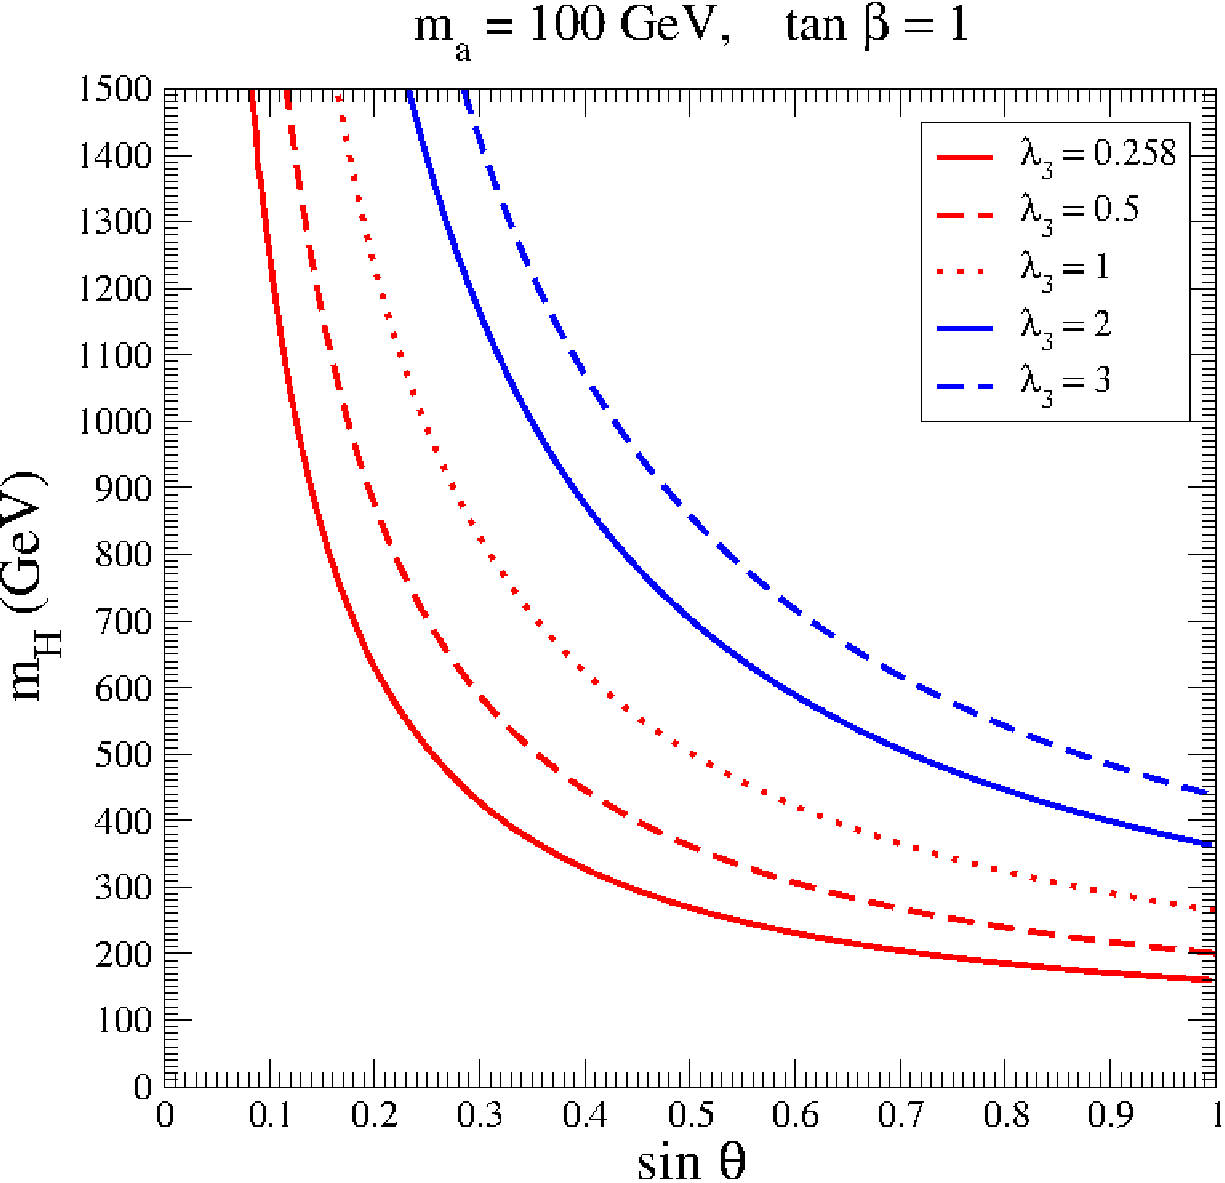
\includegraphics[width=0.485\textwidth]{texinputs/03_theoparameters/Figs/Plot_Eq.pdf}
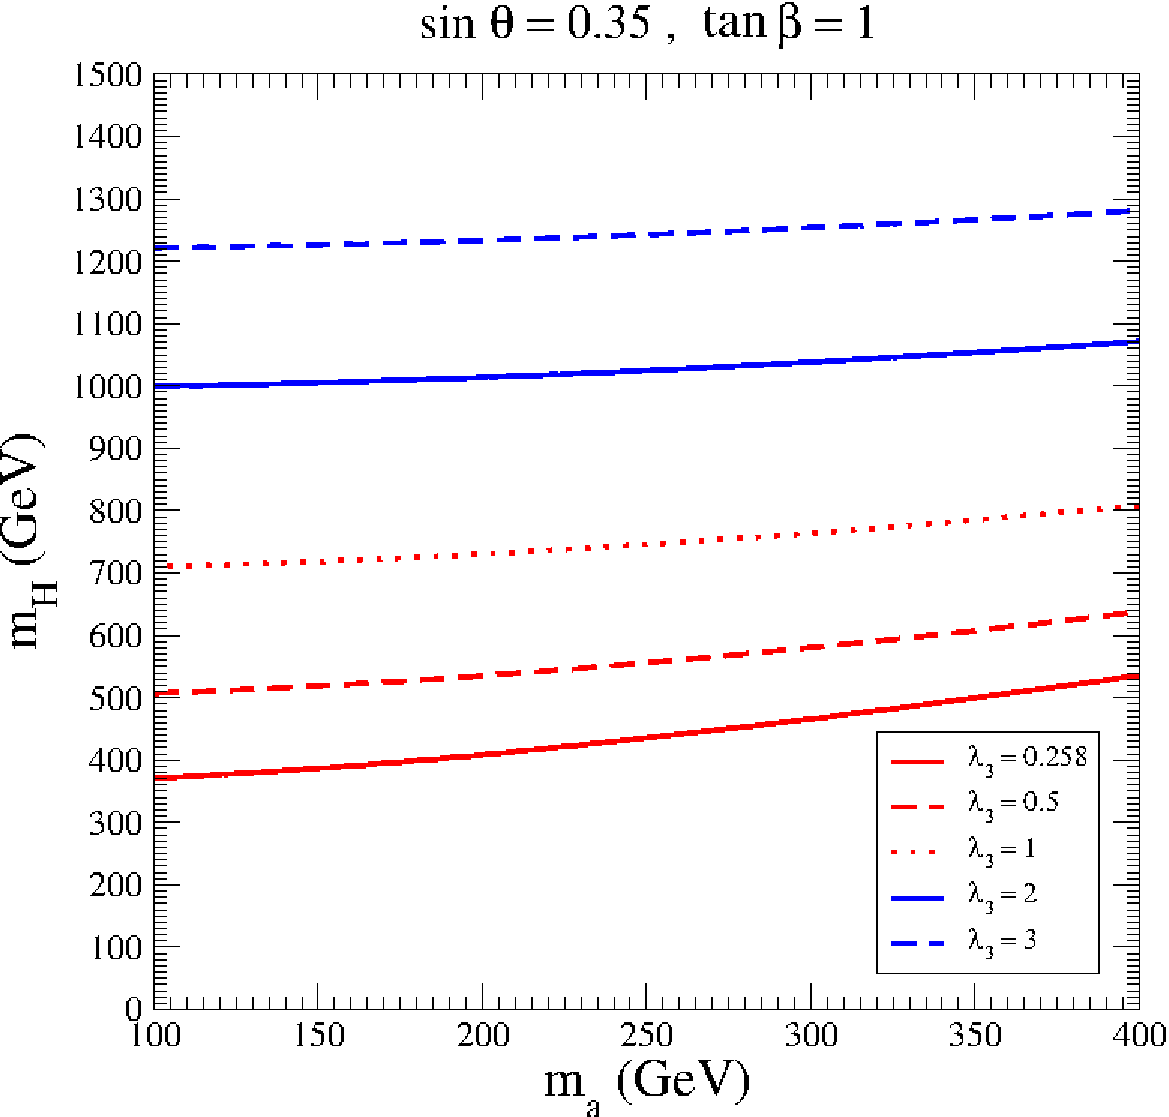
\includegraphics[width=0.485\textwidth]{texinputs/03_theoparameters/Figs/Plot_ma.pdf}
\caption{\small Regions of parameter space in the 
    ($M_a,\, M_{H}$) (left) and ($s_{\theta},\, M_a$) (right) planes for which the tree-level boundedness from below conditions~\eqref{stability2HDM} are satisfied, assuming $M_{H^{\pm}} = M_{H} = M_{A}$. \label{Fig_Stability}}
\end{center}
\vspace{-2mm}
\end{figure}
%
%
Therefore, in the benchmarks for the mono-Higgs signal $\sigma (pp \to A \to ah \to h + E_T^\text{miss})$, we consider this limit. The coupling of the heavy neutral scalar $H$ to two pseudoscalar degrees of freedom in turn is independent of $\lambda_{P_1}$ and $\lambda_{P2}$ for $\lambda_{P1}\approx \lambda_{P2}$,
    \begin{eqnarray}
     g_{Haa} &=& \frac{1}{m_{H} \,v} \left[ 2\, t_{2\beta}^{-1}\, s_{\theta}^2\, 
(m_h^2 - \lambda_3 v^2) + s_{2\beta}\, c_{\theta}^2 v^2 (\lambda_{P1} - \lambda_{P2}) \right] \nonumber \\
&\stackrel{\lambda_{P_1}\approx \lambda_{P_2}}{\longrightarrow} & \frac{1}{m_{H} \,v} \left[ 2\, t_{2\beta}^{-1}\, s_{\theta}^2\, 
(m_h^2 - \lambda_3 v^2) \right] \,. 
    \end{eqnarray}
In this limit, the partial decay width $\Gamma(H \to aa)$ is enhanced for sizable $\lambda_3$, and the branching ratio $\text{Br}(H \to aZ)$ is reduced. Searches for mono-Z final states $\sigma(pp \to H \to aZ \to Z + E_T^\text{miss})$ are therefore most sensitive if $\lambda_{P1}$ and $\lambda_{P2}$ are small or sufficiently split.

 


